\documentclass[final,a4paper,openany,12pt]{mwbk}
\usepackage{polski}
\usepackage[utf8]{inputenc}
\usepackage[T1]{fontenc}
\usepackage{lmodern}
\usepackage{microtype}

\usepackage{url}
\usepackage{algorithm}
\usepackage{algpseudocode}
\usepackage{makeidx}
\usepackage{graphicx}
%\prefixing % usunięto, bo psuje listings, a używamy utf8

\renewcommand*\listalgorithmname{Spis algorytmów\protect}

\usepackage{fancyhdr}
\pagestyle{fancy}
\fancyhf{}
\fancyhead[L]{\nouppercase{\leftmark}}
\fancyfoot[C]{\thepage}
\renewcommand{\headrulewidth}{0.4pt}
\renewcommand{\footrulewidth}{0pt}

\usepackage[hidelinks]{hyperref}
\usepackage{bookmark}
\hypersetup{
  pdfauthor={Jan Zakroczymski},
  pdftitle={FAscnn++: Rozwinięcie architektury Fast-SCNN o mechanizm Fast Attention i efektywny moduł fuzji cech w zastosowaniu segmentacji obrazów},
  pdfsubject={Praca licencjacka},
  pdfkeywords={segmentacja semantyczna, FAscnn++, FastSCNN, ENet, Cityscapes}
}

\usepackage{caption}
\usepackage{subcaption}
\usepackage{booktabs}
\usepackage{longtable}
\usepackage{tabularx}
\usepackage{array}

\usepackage{amsmath, amssymb, amsthm}
\newtheorem{definicja}{Definicja}[chapter]
\newtheorem{twierdzenie}{Twierdzenie}[chapter]
\newtheorem{wniosek}{Wniosek}[chapter]
\newtheorem{twr}{Twierdzenie}[section]

\usepackage{listings}
\lstset{
  basicstyle=\ttfamily\small,
  numbers=left,
  numberstyle=\tiny,
  stepnumber=1,
  numbersep=8pt,
  showstringspaces=false,
  tabsize=2,
  breaklines=true,
  frame=single,
  captionpos=b,
  inputencoding=utf8,
  extendedchars=true
}

\usepackage{csquotes}
\usepackage[backend=biber,style=numeric,sorting=nty]{biblatex}
\addbibresource{../rozdzialy/references.bib}
\DeclareCiteCommand{\bibref}
  {}
  {\printtext[bibhyperref]{\mkbibbrackets{\printfield{labelnumber}}}}
  {\addcomma\space}
  {}

\newcommand{\uczelnia}{UNIWERSYTET KARDYNAŁA STEFANA WYSZYŃSKIEGO\\W WARSZAWIE}
\newcommand{\wydzial}{WYDZIAŁ MATEMATYCZNO-PRZYRODNICZY\\SZKOŁA NAUK ŚCISŁYCH}
\newcommand{\kierunek}{Informatyka}
\newcommand{\miasto}{Warszawa}
\newcommand{\rok}{2026}
\newcommand{\autor}{Jan Zakroczymski}
\newcommand{\nrindeksu}{126732}
\newcommand{\promotor}{dr inż. Robert Kłopotek}
\newcommand{\tytul}{FAscnn++: Rozwinięcie architektury Fast-SCNN o mechanizm\\Fast Attention i efektywny moduł fuzji cech\\w zastosowaniu segmentacji obrazów}

% ustawienia do wydruku dwustronnego z uwzględnieniem dodatkowego miejsca na zszycie
\setlength{\oddsidemargin}{0.46cm}   %margines nieparzysty
\setlength{\evensidemargin}{-0.54cm} %margines parzysty
\setlength{\textwidth}{16cm}         %szerokość tekstu na stronie
\linespread{1.1}

\begin{document}

\begin{titlepage}
\vspace{-0.5cm}

{\centering
{\footnotesize
\begin{tabular}{c}
\uczelnia\\
\end{tabular}
}
\vspace{2.5cm}

{\footnotesize
\begin{tabular}{c}
\wydzial\\
\end{tabular}
}
\vspace{3.5cm}

\renewcommand{\arraystretch}{1.5} % zwiększamy odległość między wierszami

{\normalsize
\begin{tabular}{c}
\autor\\
Nr alb.: \nrindeksu\\
Kierunek studiów: \kierunek\\
\end{tabular}
}

\vspace{1.5cm}

{\large
\begin{tabular}{c}
\tytul\\
\end{tabular}
}

}

\renewcommand{\arraystretch}{1} % przywracamy domyślną odległość miedzy wierszami

\vspace{5cm}

\hspace{6cm}
\begin{tabular}{l}
Praca licencjacka wykonana\\
pod kierunkiem naukowym\\
\promotor
\end{tabular}

\vspace{3cm}

{\centering

{\small
\begin{tabular}{c}
{\miasto, \rok}\\
\end{tabular}
}

}
\end{titlepage}

\tableofcontents

\chapter*{Wykaz skrótów}
\addcontentsline{toc}{chapter}{Wykaz skrótów}
\begin{description}
    \item[ADAS] \textit{Advanced Driver Assistance Systems} -- zaawansowane systemy wspomagania kierowcy
    \item[AI] \textit{Artificial Intelligence} -- sztuczna inteligencja
    \item[AMP] \textit{Automatic Mixed Precision} -- automatyczna precyzja mieszana
    \item[ASPP] \textit{Atrous Spatial Pyramid Pooling} -- przestrzenne piramidalne łączenie atrusowe
    \item[CBAM] \textit{Convolutional Block Attention Module} -- splotowy moduł uwagi blokowej
    \item[CLI] \textit{Command Line Interface} -- interfejs wiersza poleceń
    \item[CNN] \textit{Convolutional Neural Network} -- konwolucyjna sieć neuronowa
    \item[CPU] \textit{Central Processing Unit} -- główna jednostka obliczeniowa (procesor)
    \item[CRF] \textit{Conditional Random Field} -- warunkowe pola losowe
    \item[DSConv] \textit{Depthwise Separable Convolution} -- splot separowalny w głąb
    \item[FCN] \textit{Fully Convolutional Network} -- w pełni konwolucyjna sieć neuronowa
    \item[FFM] \textit{Feature Fusion Module} -- moduł fuzji cech
    \item[FN] \textit{False Negative} -- fałszywie negatywna detekcja (fałszywe odrzucenie)
    \item[FP] \textit{False Positive} -- fałszywie pozytywna detekcja (fałszywy alarm)
    \item[FPN] \textit{Feature Pyramid Network} -- piramidalna sieć cech
    \item[FPS] \textit{Frames Per Second} -- liczba klatek na sekundę
    \item[GFLOPs] \textit{Giga Floating Point Operations} -- miliardy operacji zmiennoprzecinkowych (miara złożoności modelu)
    \item[GPU] \textit{Graphics Processing Unit} -- jednostka przetwarzania graficznego
    \item[IoT] \textit{Internet of Things} -- Internet rzeczy
    \item[IoU] \textit{Intersection over Union} -- miara pokrycia predykcji z wzorcem (przecięcie przez sumę)
    \item[LR] \textit{Learning Rate} -- współczynnik uczenia
    \item[mIoU] \textit{mean Intersection over Union} -- uśredniona wartość miary IoU dla wszystkich klas
    \item[MLP] \textit{Multi-Layer Perceptron} -- wielowarstwowy perceptron
    \item[NAS] \textit{Neural Architecture Search} -- automatyczne wyszukiwanie architektury sieci neuronowej
    \item[PA] \textit{Pixel Accuracy} -- dokładność pikselowa
    \item[R\&D] \textit{Research and Development} -- badania i rozwój
    \item[SGD] \textit{Stochastic Gradient Descent} -- stochastyczny spadek wzdłuż gradientu
    \item[SOTA] \textit{State of the Art} -- najnowocześniejsze osiągnięcia w dziedzinie
    \item[TP] \textit{True Positive} -- prawdziwie pozytywna detekcja
    \item[UAV] \textit{Unmanned Aerial Vehicle} -- bezzałogowy statek powietrzny (dron)
\end{description}
% \listoffigures
% \listoftables
% \lstlistoflistings

\chapter*{Streszczenie}
\addcontentsline{toc}{chapter}{Streszczenie}
Praca przedstawia projekt i ocenę architektury FAscnn++ do semantycznej segmentacji obrazów w czasie rzeczywistym. 
Głównym celem badań jest analiza kompromisu pomiędzy dokładnością segmentacji a wydajnością obliczeniową lekkiej architektury wielostrumieniowej rozszerzonej o moduły uwagi. 
Eksperymenty przeprowadzono na zbiorze danych Cityscapes. Część teoretyczna obejmuje przegląd ograniczeń modeli czasu rzeczywistego oraz architektur referencyjnych. 
W części praktycznej opisano implementację sieci, konfigurację środowiska testowego oraz ewaluację modelu FAscnn++. Analizie poddano kluczowe metryki jakości (mIoU, dokładność pikselowa) oraz wskaźniki przepustowości (FPS, opóźnienie inferencji).

\textbf{Słowa kluczowe:} segmentacja semantyczna; FAscnn++; Cityscapes; architektury lekkie; czas rzeczywisty.

\chapter{Wstęp}

Semantyczna segmentacja obrazów jest kluczowym problemem w dziedzinie widzenia maszynowego \bibref{minaee2021image}. Klasyfikacja obiektów na poziomie pojedynczych pikseli umożliwia precyzyjną interpretację przestrzenną sceny. Ma to krytyczne znaczenie dla działania systemów ADAS \bibref{feng2020deep}, autonomicznych bezzałogowców \bibref{osco2021review} oraz robotyki mobilnej \bibref{garg2020semantics}.

W zastosowaniach czasu rzeczywistego (np. autonomiczna nawigacja w scenach miejskich) modele wizyjne muszą rozpoznawać wiele złożonych klas (infrastruktura drogowa, piesi, pojazdy) z ułamkowym opóźnieniem. Głównym wyzwaniem projektowym w tym obszarze jest optymalizacja kompromisu pomiędzy dokładnością predykcji a narzutem obliczeniowym sieci splotowej.

Głębokie modele segmentacyjne o wysokiej precyzji, takie jak SETR \bibref{zheng2021rethinking} czy Mask2Former \bibref{cheng2022masked}, charakteryzują się potężną złożonością matematyczną. Całkowicie dyskwalifikuje je to z bezpośrednich wdrożeń brzegowych (edge computing). Praktycznym rozwiązaniem są wysoce zoptymalizowane, lekkie architektury splotowe, w tym ENet \bibref{paszke2016enet} i Fast-SCNN \bibref{poudel2019fast}, ukierunkowane na drastyczną minimalizację liczby parametrów. Poprawa precyzji działania takich architektur, przy zachowaniu bezkompromisowej przepustowości, pozostaje w centrum aktualnych prac badawczych.

Celem pracy jest projekt, oprogramowanie i rygorystyczna ewaluacja rozszerzeń dla architektury Fast-SCNN. Skonstruowano model FAscnn++, łączący strukturę wielostrumieniową z wydajnymi mechanizmami uwagi. Przygotowane rewizje sieci przetestowano i porównano analitycznie z modelami referencyjnymi na zbiorze Cityscapes \bibref{cordts2016cityscapes}.

Hipoteza badawcza zakłada, że integracja modułów uwagi ze sprawdzoną topologią splotową w modelu FAscnn++ znacząco zwiększy metrykę dokładności (mIoU) względem innych modeli klasy lekkiej. Zostanie to osiągnięte przy utrzymaniu przepustowości klatek (FPS) kompatybilnej z systemami o reżimie czasu rzeczywistego. Poprawność tej tezy zweryfikowano wykorzystując ustrukturyzowany pakiet miar jakości (mIoU, Pixel Accuracy) oraz miar wydajności (FPS, latency, GFLOPs, liczba parametrów).

Struktura dysertacji: Rozdział 2 formułuje wprost problem badawczy. Rozdział 3 dokumentuje autorską implementację programową. W rozdziale 4 sformalizowano metodologię i warunki środowiska testowego. Rozdział 5 to szczegółowa i analityczna ewaluacja uzyskanych wyników. Pracę zamyka wykaz kluczowych konkluzji (Rozdział 6).

\chapter{Przedstawienie problemu badawczego}

\section{Definicja problemu}
Problem badawczy dotyczy semantycznej segmentacji scen miejskich w czasie rzeczywistym. Zadanie polega na przypisaniu każdemu pikselowi obrazu o wymiarach $H \times W$ etykiety klasy semantycznej. Kluczowym aspektem pracy jest optymalizacja kompromisu pomiędzy dokładnością predykcji a narzutem obliczeniowym. Szybkość wnioskowania determinuje użyteczność modelu w systemach takich jak ADAS czy robotyka mobilna. Wysoka przepustowość (FPS) umożliwia szybszą nawigację i krótszy czas reakcji na przeszkody.

\section{Znaczenie ograniczeń wydajnościowych}
Wiele współczesnych modeli segmentacji osiąga wysoką dokładność kosztem dużej liczby parametrów, obciążenia pamięci oraz długiego czasu inferencji. Ogranicza to ich wdrożenie na platformach brzegowych (Edge AI). Z tego względu ewaluacja obejmuje zarówno jakość predykcji, jak i opóźnienie (latency). W zastosowaniach takich jak ADAS, bezzałogowce i robotyka, opóźnienie stanowi parametr krytyczny. Standardy inżynierskie często definiują czas rzeczywisty jako przepustowość powyżej 30 FPS \bibref{elhassan2024real}. W aplikacjach wymagających dynamicznej pętli sprzężenia zwrotnego (np. \textit{visual servoing}) celuje się w 60 Hz \bibref{corke1989videorate}. Wymagania te zależą ściśle od użytego sprzętu i dynamiki otoczenia.

\section{Podstawy teoretyczne}

\subsection{Sieci konwolucyjne}
Podstawowym modułem w modelach wizyjnych są konwolucyjne sieci neuronowe (CNN), zbudowane z warstw splotowych i nieliniowych aktywacji. W niniejszej pracy analizowane są wyłącznie warianty architektur splotowych optymalizowane pod kątem wysokiej wydajności.

\subsection{Zaawansowane bloki architektoniczne}
Optymalizacja architektur CNN wymaga modyfikacji strukturalnych, z których kluczowe to konwolucje separowalne, bloki typu \textit{bottleneck} oraz przetwarzanie wieloskalowe.

\paragraph{Konwolucje separowalne (Depthwise Separable Convolutions)}
Tradycyjny splot (jądro $D_K \times D_K$, $M$ kanałów wejściowych, $N$ wyjściowych, rozdzielczość mapy $D_F \times D_F$) wiąże się z kosztem obliczeniowym:
$$ C_{std} = D_K \cdot D_K \cdot M \cdot N \cdot D_F \cdot D_F $$
Konwolucja separowalna \bibref{howard2017mobilenets, chollet2017xception} rozdziela tę operację na splot przestrzenny (\textit{depthwise}) i punktowy (\textit{pointwise}). Koszt wynosi wówczas:
$$ C_{sep} = D_K \cdot D_K \cdot M \cdot D_F \cdot D_F + M \cdot N \cdot D_F \cdot D_F $$
Mechanizm ten drastycznie kompresuje model, osiągając współczynnik redukcji operacji równy $\frac{1}{N} + \frac{1}{D_K^2}$.

\paragraph{Moduły wąskiego gardła (\textit{Bottleneck})}
W sieciach takich jak ResNet \bibref{he2016deep} moduły wąskiego gardła zapobiegają eksplozji parametrów w głębokich warstwach. Dane $x \in \mathbb{R}^{H \times W \times C}$ podlegają rzutowaniu do niższej wymiarowości (kompresja), splotowi przestrzennemu, a następnie ekspansji kanałowej:
$$ F(x) = W_{1\times1}^{out} * \sigma\left( W_{3\times3} * \sigma\left( W_{1\times1}^{in} * x \right) \right) $$
Liczba kanałów filtru $W_{1\times1}^{in}$ jest znacznie mniejsza niż $C$, co pozwala na oszczędność pamięci i mocy obliczeniowej.

\subsubsection{Mechanizmy uwagi i ich koszt obliczeniowy}
W konwencjonalnych sieciach CNN wagi filtrów są statyczne niezależnie od lokalizacji. Mechanizmy uwagi (\textit{attention}) umożliwiają dynamiczne ważenie cech, wzmacniając zdolności reprezentacyjne sieci przy minimalnym pogłębianiu architektury.

\paragraph{Uwaga kanałowa i przestrzenna}
Moduł \textit{Squeeze-and-Excitation} (SE) wdrożony w sieciach SENet \bibref{hu2018squeeze} agreguje informację przestrzenną poprzez \textit{Global Average Pooling}. Wynik przetwarzany jest przez dwuwarstwowy perceptron (MLP), generując wektor wag $\alpha \in \mathbb{R}^C$. Kanały macierzy cech $X$ są następnie skalowane:
$$ X'_{c} = \alpha_c \cdot X_c $$
Moduł CBAM \bibref{woo2018cbam} rozszerza to rozwiązanie, aplikując sekwencyjnie uwagę kanałową oraz przestrzenną. Koszt tych mechanizmów to ułamek procenta całkowitej wartości GFLOPs modelu.

\subsection{Samouwaga (Self-Attention) i bloki nielokalne}
Koncepcja architektury Transformer \bibref{vaswani2017attention} została przeniesiona do sieci CNN w formie bloków nielokalnych (\textit{Non-local Neural Networks}) \bibref{wang2018nonlocal}. Dla wektora wejściowego rzutowanego na macierze zapytań ($Q$), kluczy ($K$) i wartości ($V$), operacja atencji oblicza wagowaną sumę:
$$ \text{Attention}(Q, K, V) = \text{softmax}\left(\frac{QK^T}{\sqrt{d_k}}\right)V $$
gdzie $d_k$ to współczynnik skalujący.

\paragraph{Złożoność obliczeniowa samouwagi}
Złożoność klasycznej samouwagi zależy od rozdzielczości obrazu. Dla mapy cech o liczbie pikseli $N = H \times W$ i wymiarze $C$, obliczenie macierzy podobieństwa $QK^T$ wymaga $\mathcal{O}(N^2 C)$ operacji. Całkowita złożoność wynosi \bibref{dosovitskiy2020image}:
$$ \mathcal{O}(N^2 C) = \mathcal{O}(H^2 \cdot W^2 \cdot C) $$
Zależność kwadratowa od rozdzielczości wyklucza zastosowanie tego mechanizmu na wczesnych etapach sieci (duże $H$ i $W$). Narzędzie to stosuje się po wstępnej redukcji cech lub z wykorzystaniem uwagi lokalnej (np. Swin Transformer \bibref{liu2021swin}).

\paragraph{Mechanizmy uwagi w segmentacji}
Uwaga globalna poprawia dokładność segmentacji poprzez modelowanie rozległego kontekstu sceny \bibref{hu2020fastattention}. Ograniczeniem pozostaje operacja Softmax z kwadratową złożonością przestrzenną $\mathcal{O}(n^2c)$ (gdzie $n = H \times W$) \bibref{hu2020fastattention}. Blokuje to implementację klasycznej atencji w systemach czasu rzeczywistego, dla których analiza pełnej klatki wideo jest konieczna.

\paragraph{Rozwiązania dla ograniczeń sprzętowych}
Skuteczną alternatywą jest mechanizm szybkiej uwagi (\textit{Fast Attention}) \bibref{hu2020fastattention}. Eliminacja normalizacji Softmax na rzecz miary podobieństwa kosinusowego pozwala na rearanżację kolejności mnożenia macierzy. Złożoność operacji maleje do wymiaru liniowego $\mathcal{O}(nc^2)$ \bibref{hu2020fastattention}. W zadaniach wizyjnych ($n \gg c$) mechanizm ten ekstrahuje nielokalny kontekst przy ułamkowym koszcie względem klasycznej atencji.

\subsection{Segmentacja semantyczna, panoptyczna i instancyjna}
Wizja komputerowa wyróżnia segmentację semantyczną (klasyfikacja pikseli) \bibref{long2015fully}, instancyjną (identyfikacja odrębnych obiektów) \bibref{he2017mask} oraz panoptyczną (połączenie obu metod) \bibref{kirillov2019panoptic}. Praca koncentruje się na segmentacji semantycznej, dostarczającej ogólnego opisu sceny, wymaganego do autonomicznej nawigacji w reżimie niskich opóźnień inferencji.

\subsection{Klasyczne modele segmentacji}
Pionierskim rozwiązaniem w dziedzinie są sieci FCN \bibref{long2015fully}. Inne klasyczne struktury, jak U-Net \bibref{ronneberger2015u}, SegNet \bibref{badrinarayanan2017segnet}, DeepLab \bibref{chen2018deeplab} oraz PSPNet \bibref{zhao2017pspnet}, osiągają dużą celność. Z uwagi na wysokie zapotrzebowanie na GFLOPs są nieużyteczne na platformach brzegowych. Ich dedykowanym zamiennikiem dla systemów mobilnych stała się sieć ICNet \bibref{zhao2018icnet}.

\subsection{Typy architektur}

\paragraph{Enkoder-dekoder}
Architektury sekwencyjne (np. U-Net \bibref{ronneberger2015u}) realizują rekonstrukcję z użyciem połączeń omijających (\textit{skip connections}). Koszt obliczeniowy wymusza ich odrzucenie z aplikacji czasu rzeczywistego.

\paragraph{Wielogałęziowe i wielorozdzielcze}
Systemy w rodzaju ICNet \bibref{zhao2018icnet} czy Lite-HRNet \bibref{yu2021lite} przetwarzają obraz równolegle w wielu rozdzielczościach. Ekstrakcja kontekstu odbywa się na silnie skompresowanych mapach, a odtwarzanie detali na płytkich warstwach o szerokiej przestrzeni.

\paragraph{Dwuścieżkowe i wielościeżkowe}
Modele brzegowe opierają się na dekompozycji przetwarzania. Sieć BiSeNet \bibref{yu2018bisenet, yu2021bisenetv2} rozdziela ścieżkę przestrzenną i kontekstową. Konstrukcje DDRNet \bibref{hong2021deep} oraz PIDNet \bibref{xu2023pidnet} rozbudowują tę ideę o gęstą fuzję sygnału. Takie ujęcie stanowi architektoniczny fundament proponowanego modelu FAscnn++.

\section{Przegląd architektur efektywnych i mechanizmów uwagi}

\paragraph{Pierwsza generacja i podejścia wieloskalowe}
Wczesne modele (ENet \bibref{paszke2016enet}, ESPNetv2 \bibref{mehta2019espnetv2}) optymalizowały obciążenie sprzętowe kompresując kanały i aplikując asymetryczne sploty. Kosztem była utrata detali. Architektura Fast-SCNN \bibref{poudel2019fastscnn} z wbudowanym modułem kaskadowym (\textit{Learning to Downsample}) ustaliła standard wydajności (123 FPS) w formacie $1024 \times 2048$. Fast-SCNN służy jako główny punkt referencyjny niniejszej pracy.

\paragraph{Nowoczesne architektury wielościeżkowe}
Współczesne sieci SOTA odseparowują ścieżkę detali od kontekstu (BiSeNetV2, STDC2). DDRNet-23-slim pozwala na 77,4\% mIoU przy 102 FPS. Architektura PIDNet-S notuje 78,6\% mIoU (93,2 FPS). Ich implementacja dla urządzeń o ścisłym reżimie energetycznym pozostaje niemożliwa. Nowsze modele ograniczają opóźnienia poprzez skracanie dekoderów (PP-LiteSeg-T). Model LCNet3\_7 redukuje wielkość do 0,51 miliona parametrów zachowując 73,8\% mIoU. Układ ISANet podnosi mIoU do 76,7\% (1,37 M parametrów). Nowatorska sieć GCNet poprzez reparametryzację uzyskuje 77,3\% mIoU i rekordowe 193,3 FPS w natywnej rozdzielczości $1024 \times 2048$.

\paragraph{Transformery wizyjne, szybka uwaga (Fast Attention) i modele hybrydowe}
Transformery wizyjne redukują operacje uwagi wykorzystując warianty strukturalne: EfficientViT \bibref{liu2023efficientvit}, TopFormer-T, SeaFormer-S/T oraz systemy hybrydowe (MobileViT \bibref{mehta2022mobilevit}). Sieć LMIINet łączy splot i atencję, zapewniając 72,0\% mIoU na zaledwie 0,72 M parametrach i przy obciążeniu 11,74 GFLOPs. Model RTLinearFormer (2025) stosuje uwagą liniową, notując płynność 66,7 FPS przy 78,41\% mIoU.
Algorytmem krytycznym dla badanego obszaru jest mechanizm modelu FANet \bibref{hu2020fanet}. Zmiana operacji Softmax na \textit{cosine similarity} zapewnia liniową kalkulację uwagi ($\mathcal{O}(nc^2)$). Kluczowe dane ewaluacyjne dla modelu FAscnn++\_V18 i sieci referencyjnych zamieszczono w Tabeli \ref{tab:architektury}.

\section{Luka badawcza}
Rynek systemów wizyjnych jest silnie spolaryzowany. Wysoce precyzyjne sieci (PIDNet \bibref{xu2023pidnet}, DDRNet \bibref{hong2021ddrnet}, GCNet) wymagają infrastruktury wielkości 20--100 GFLOPs, wykluczając instalacje w lekkich jednostkach (UAV). Z kolei modele z segmentu \textit{ultra-lightweight} (PP-LiteSeg-T1 \bibref{peng2022ppliteseg}, STDC2-Seg50 \bibref{fan2021stdc}, LCNet3\_7 \bibref{shi2024lcnet}) osiągają płynność kosztem kompresji klatki do formatów podrzędnych (np. $512 \times 1024$). Generuje to utratę kluczowych detali krawędzi i spadki precyzji w obrębie małych obiektów.

Wymuszenie obsługi klatek w rozmiarze natywnym ($1024 \times 2048$) prowadzi do utraty parametrów pracy. TopFormer-T \bibref{zhang2022topformer} oferuje $\sim$100 FPS (RTX 3090) z bardzo słabym wynikiem 70,70\% mIoU. Sieć SeaFormer-S \bibref{wan2023seaformer} gwarantuje 76,10\% mIoU, ale z płynnością jedynie 7,6 FPS na urządzeniach mobilnych.

Zidentyfikowana luka sprzętowa i algorytmiczna dowodzi braku architektury konwolucyjnej, która jednocześnie:
\begin{itemize}
    \item \textbf{Przełamuje kompromis rozdzielczości:} przetwarza niezmodyfikowane wideo w jakości $1024 \times 2048$ zachowując zapotrzebowanie do 10 GFLOPs i budżet do 1,2 miliona parametrów.
    \item \textbf{Gwarantuje dokładność krytyczną:} osiąga jakość przekraczającą 65\% mIoU na zbiorze Cityscapes przy zachowaniu rozdzielczości rzędu natywnego.
    \item \textbf{Oferuje elastyczne środowisko dla badań (Edge AI):} posiada wdrożenia pozwalające na bezkompromisowe badania ablacyjne dla nowo projektowanych modułów sprzętowych.
\end{itemize}

\section{Sformułowanie problemu badawczego}
Celem naukowym pracy jest wdrożenie elastycznej architektury wpasowującej się w powyższą lukę. Problem sprowadzono do weryfikacji pytań badawczych:
\begin{itemize}
    \item Czy topologiczna poprawa układów z rodziny Fast-SCNN (jako wariant FAscnn++) oferuje zoptymalizowany stosunek mIoU do GFLOPs dla predykcji pełnoklatkowej ($1024 \times 2048$) w odniesieniu do sieci \textit{ultra-lightweight}?
    \item Jak zdefiniowane mechanizmy splotowe wpływają na narzut strukturalny i jakość klasyfikacji poszczególnych klas?
    \item Czy dodatkowe zużycie pasma pamięci wbudowanej (\textit{memory bandwidth}) w ramach mechanizmów Fast Attention uniemożliwi płynne działanie sieci utrzymanej w restrykcjach $<10$ GFLOPs?
\end{itemize}

\chapter{Implementacja}

\section{Architektura systemu i struktura projektu}
Zaprojektowany system posiada strukturę modularną, co ułatwia integrację nowych modeli i modyfikację parametrów treningowych bez ingerencji w rdzeń aplikacji. Drzewo katalogów odzwierciedla podział na moduły logiczne:
\begin{itemize}
    \item \texttt{src/data/} – definicje zbiorów danych (m.in. \texttt{Cityscape.py}) oraz logika transformacji i augmentacji.
    \item \texttt{src/model\_architecture/} – moduł sieci neuronowych. Podkatalog \texttt{FAscnn++/} grupuje warianty architektoniczne (od V1 do V31). Plik \texttt{model\_factory.py} dostarcza klasę \texttt{ModelBuilder} opartą na wzorcu projektowym fabryki.
    \item \texttt{src/utils/} – komponenty pętli treningowej (\texttt{train.py}), procedury ewaluacyjne (\texttt{test.py}), implementacje funkcji strat (\texttt{loss.py}) oraz kalkulatory metryk (\texttt{metrics.py}).
    \item \texttt{src/\_\_main\_\_.py} – główny punkt wejścia aplikacji (CLI), integrujący moduły i parsujący konfigurację.
    \item \texttt{visualisation/} – zbiór skryptów generujących wizualizacje predykcji oraz wykresy ewaluacyjne.
\end{itemize}

\section{Technologie i wymagania systemowe}
Aplikację zaimplementowano w języku Python \bibref{van1995python} (wersja $\ge$ 3.8). Silnikiem obliczeniowym dla sieci neuronowych jest biblioteka PyTorch \bibref{paszke2019pytorch} (wersja 2.1), gwarantująca akcelerację sprzętową GPU poprzez biblioteki CUDA.

Kluczowe zależności środowiskowe obejmują:
\begin{itemize}
    \item \texttt{torch} (2.10.0) – framework obliczeniowy operujący na tensorach.
    \item \texttt{numpy} (2.4.1) – wysokowydajne operacje macierzowe.
    \item \texttt{matplotlib} (3.10.8) – silnik wizualizacji danych.
    \item \texttt{PyYAML} (6.0.3) – parser plików konfiguracyjnych.
    \item \texttt{einops} (0.8.2) – elastyczne operacje tensorowe, wykorzystywane w implementacji mechanizmów uwagi.
    \item \texttt{tqdm} (4.67.1) – wskaźniki postępu dla CLI.
    \item \texttt{tensorboard} (2.20.0) – platforma logowania metryk treningowych.
\end{itemize}

\section{Opis kluczowych komponentów}

\subsection{Moduł danych i augmentacja}
Klasa \texttt{CityscapesDataModule} (\texttt{src/data/Cityscape.py}) implementuje potok ładowania zestawu Cityscapes. Do jej zadań należą:
\begin{itemize}
    \item mapowanie identyfikatorów zbioru źródłowego na 19 klas treningowych,
    \item augmentacja strumieniowa (ang. \textit{on-the-fly}): losowe skalowanie, przycinanie (\textit{random crop}), lustrzane odbicia horyzontalne (\textit{horizontal flip}) i modyfikacje jasności,
    \item transformacja do formatu tensora i normalizacja wejścia w oparciu o statystyki bazy ImageNet.
\end{itemize}

\subsection{Fabryka modeli – ModelBuilder}
Klasa \texttt{ModelBuilder} (\texttt{src/model\_architecture/model\_factory.py}) odpowiada za instancjonowanie architektur sieci. Abstrakcja ta obsługuje modele referencyjne (ENet \bibref{paszke2016enet}, Fast-SCNN \bibref{poudel2019fastscnn}) oraz wszystkie warianty rodziny FAscnn++. Instancjonowanie konkretnej topologii wymaga jedynie modyfikacji odpowiedniego parametru w pliku konfiguracyjnym.

\subsection{Pętla treningowa i ewaluacja}
Funkcja \texttt{train\_main} (\texttt{src/utils/train.py}) obsługuje cykl życia procesu uczenia:
\begin{itemize}
    \item alokację optymalizatora (SGD z parametrem \textit{momentum}) i harmonogramu współczynnika uczenia (\texttt{PolyLR}),
    \item akcelerację obliczeń dzięki zastosowaniu mieszanej precyzji zmiennoprzecinkowej (AMP – \textit{Automatic Mixed Precision}),
    \item synchronizację z platformą TensorBoard w celu logowania przebiegu funkcji straty oraz metryk mIoU i Pixel Accuracy,
    \item automatyczną serializację punktów kontrolnych modelu (wagi \textit{best.pt} i \textit{last.pt}).
\end{itemize}

\section{Konfiguracja i automatyzacja eksperymentów}
Zarządzanie parametrami eksperymentów realizowane jest za pośrednictwem pliku \texttt{config.yaml}, co zapewnia reprodukowalność procedur ewaluacyjnych. Struktura konfiguracji dzieli się na sekcje:
\begin{itemize}
    \item \texttt{training}: hiperparametry optymalizacyjne (LR, batch size, liczba epok), definicje ścieżek dostępu i warianty augmentacji.
    \item \texttt{test}: rozdzielczość wejściowa dla ewaluacji i liczba generowanych wizualizacji.
    \item \texttt{model}: deskryptor wybranej topologii sieci oraz liczba obsługiwanych klas.
    \item \texttt{patch}: parametry opcjonalnego kafelkowania klatek (ang. \textit{patching}).
\end{itemize}

Przygotowano również zbiór skryptów powłoki (\texttt{.sh}) automatyzujących rutynowe procesy:
\begin{itemize}
    \item \texttt{setup.sh} – budowa środowiska wirtualnego (\textit{venv}) i instalacja bibliotek.
    \item \texttt{run\_train.sh} – inicjalizacja potoku treningowego z domyślną parametryzacją.
    \item \texttt{run\_test.sh} – egzekucja walidacji skuteczności modelu na dedykowanym zbiorze danych.
\end{itemize}

\section{Interfejs użytkownika (CLI)}
Aplikacja udostępnia interfejs wiersza poleceń (CLI), pozwalający na nadpisywanie parametrów środowiskowych. Przykłady wywołań:
\begin{itemize}
    \item \textbf{Trenowanie modelu:} \\
    \texttt{python -m src train --config config.yaml --model FAscnn++\_V13 --batch-size 8}
    \item \textbf{Testowanie i ewaluacja:} \\
    \texttt{python -m src test --config config.yaml --model FAscnn++\_V13}
\end{itemize}
Wykorzystanie biblioteki \texttt{argparse} umożliwia nadpisywanie wartości parametrów z pliku YAML bezpośrednio w argumentach wywołania, co znacznie usprawnia proces optymalizacji hiperparametrów.

\chapter{Metodologia badań}

\section{Cel badań i pytania badawcze}
Głównym celem pracy jest implementacja i ewaluacja optymalizacji dla referencyjnej architektury Fast-SCNN. Wprowadzone ulepszenia (oznaczone jako model FAscnn++) dedykowane są systemom segmentacji semantycznej czasu rzeczywistego. Badania koncentrują się na maksymalizacji dokładności klasyfikacji (mIoU) przy jednoczesnym utrzymaniu wysokiej przepustowości (FPS) i niskiego opóźnienia inferencji (latency).

W ramach eksperymentów zestawia się wydajność modeli z rodziny FAscnn++ z referencyjnymi architekturami ENet oraz Fast-SCNN, zachowując ujednolicone warunki uczenia i tożsame środowisko sprzętowe.

Na podstawie analizy wyników sformułowano odpowiedzi na pytania badawcze:
\begin{enumerate}
    \item Czy wdrożenie zmodyfikowanej fuzji dwustrumieniowej w architekturze Fast-SCNN zwiększa precyzję segmentacji (mIoU) przy zachowaniu porównywalnego narzutu obliczeniowego?
    \item W jakim stopniu mechanizm \texttt{FastAttention} zintegrowany ze ścieżką kontekstową przewyższa klasyczne moduły \textit{Global Average Pooling} w klasyfikacji obiektów o dużej wariancji skali?
\end{enumerate}

\section{Zbiór danych}
Eksperymenty oparto na zbiorze \textit{Cityscapes Dataset} \bibref{cordts2016cityscapes}, stanowiącym standard w ewaluacji modeli wizyjnych dla systemów autonomicznych. Zbiór oferuje gęste adnotacje pikselowe obrazów zarejestrowanych w 50 miastach europejskich.

\paragraph{Charakterystyka i struktura zbioru}
Baza obejmuje 5000 obrazów w rozdzielczości $2048 \times 1024$ pikseli z precyzyjnymi maskami (\textit{fine annotations}). Zestaw podzielono na:
\begin{itemize}
    \item \textbf{Zbiór treningowy:} 2975 obrazów wykorzystywanych do optymalizacji wag sieci.
    \item \textbf{Zbiór walidacyjny:} 500 obrazów do monitorowania metryki mIoU i strojenia hiperparametrów.
    \item \textbf{Zbiór testowy:} 1525 obrazów z maskami niejawnymi, służących do końcowej ewaluacji po stronie serwera projektowego.
\end{itemize}

\paragraph{Klasyfikacja i trudności badawcze}
Procedura ewaluacyjna wyodrębnia 19 klas krytycznych dla nawigacji w ruchu miejskim. Obejmują one kategorie infrastruktury drogowej (jezdnia, chodnik), uczestników ruchu (pieszy, rowerzysta), pojazdów (samochód, autobus) oraz elementów statycznych (budynek, ogrodzenie). 

Głównym problemem analitycznym zestawu jest silne niezbalansowanie klas (\textit{class imbalance}). Dominują klasy tła (droga, niebo, budynki), natomiast obiekty takie jak motocykl czy sygnalizacja świetlna zajmują ułamkową powierzchnię kadrów. Wymusza to zastosowanie na etapie treningu technik kompensujących dominację długiego ogona, aby umożliwić modelowi ekstrakcję cech rzadkich obiektów bez obniżenia przepustowości FPS.

\paragraph{Przetwarzanie i augmentacja danych}
W celu poprawy generalizacji zaimplementowano strumieniowy potok augmentacji danych (\textit{on-the-fly}):
\begin{itemize}
    \item \textbf{Losowe skalowanie:} ze współczynnikiem w zakresie od 0,5 do 2,0 rozdzielczości bazowej.
    \item \textbf{Przycinanie (Random Crop):} do docelowego formatu $1024 \times 2048$ pikseli (lub skompresowanego, zależnie od specyfikacji testu).
    \item \textbf{Odbicie lustrzane:} horyzontalne (\textit{horizontal flip}) z prawdopodobieństwem 0,5.
    \item \textbf{Augmentacja Copy-Paste:} algorytm niwelujący problem \textit{long tail}. System losowo wyodrębnia rzadkie klasy z obrazów dawców i implementuje je na tło docelowe. Operacja ta zwiększa ekspozycję mało reprezentowanych kategorii w procesie uczenia bez ingerencji w globalny kontekst.
    \item \textbf{Normalizacja:} zgodna ze średnią wyliczoną dla zbioru ImageNet, przyspieszająca konwergencję gradientu.
\end{itemize}
W trybie inferencji modele ewaluowano na pełnych klatkach $2048 \times 1024$.

\paragraph{Kryteria doboru klas do augmentacji Copy-Paste}
Wyodrębnienie celów dla techniki Copy-Paste zrealizowano metodą ilościową (\textit{Data-Driven Copy-Paste}). Dla klasy $i$ wyznaczono metryki:
\begin{enumerate}
    \item \textbf{Globalne prawdopodobieństwo wystąpienia} ($P_{glob, i}$), definiujące udział pikseli klasy w zbiorze treningowym:
    \begin{equation}
        P_{glob, i} = \left( \frac{C_i}{T_{pixels}} \right) \cdot 100\%
    \end{equation}
    gdzie $C_i$ to suma pikseli klasy $i$, a $T_{pixels}$ oznacza łączną liczbę pikseli w zestawie uczącym.
    
    \item \textbf{Warunkowe pokrycie obrazu} ($A_{cond, i}$), szacujące powierzchnię zajmowaną przez obiekt przy jego wystąpieniu:
    \begin{equation}
        A_{cond, i} = \left( \frac{C_i / N_i}{P_{img}} \right) \cdot 100\%
    \end{equation}
    gdzie $N_i$ to liczba wystąpień obrazów z klasą $i$, a $P_{img}$ odpowiada liczbie pikseli na obraz.
\end{enumerate}

Procedurę zaaplikowano z ograniczeniem progowym: $P_{glob, i} < 1,0\%$ i $A_{cond, i} < 1,0\%$. Skutkuje to kwalifikacją wyłącznie obiektów rzadkich i małogabarytowych (światła, znaki, motocykle, rowery). Takie ujęcie zapobiega modyfikacjom przestrzennym ingerującym w topologię otoczenia ustrukturyzowanego.

\section{Modele uwzględnione w eksperymentach}
Ocenie poddano zbiór następujących wariantów sieci neuronowych:
\begin{itemize}
  \item architektury bazowe: Fast-SCNN, ENet (wraz ze skróconymi wariantami ENetv2, ENetv3),
  \item cykl ewolucyjny środowiska FAscnn++,
  \item docelowy model po przeprowadzeniu testów ablacyjnych (FAscnn++\_V18).
\end{itemize}
Wykorzystanie ENet oraz Fast-SCNN pozwala na standaryzowane, weryfikowalne zestawienie wydajności względem dotychczasowych rozwiązań brzegowych.

\section{Warunki środowiska eksperymentalnego}
Proces badawczy zrealizowano w ujednoliconym środowisku obliczeniowym. Wdrożono rygorystyczną standaryzację hiperparametrów treningowych w celu zapewnienia wiarygodności wahań celności przypisywanych cechom architektonicznym modeli.

\paragraph{Parametry treningowe}
Wszystkie sieci poddano optymalizacji przez 200 epok. Użyto optymalizatora SGD ze zmienną pędu (\textit{momentum}) ustaloną na 0,9 oraz parametrem spadku wag (\textit{weight decay}) równym $4 \times 10^{-5}$. Zaimplementowano politykę harmonogramu uczenia \textit{Poly Learning Rate}: $lr = lr_{base} \times (1 - \frac{iter}{max\_iter})^{power}$, przyjmując początkowy współczynnik uczenia $lr_{base} = 0,045$ oraz potęgę $power = 0,9$, wzorowaną na parametrach bazowych dla Fast-SCNN \bibref{poudel2019fastscnn}. 

Paczka treningowa (\textit{batch size}) zawierała 6 obrazów. Dla architektur generujących wysoki zrzut z pamięci zaaplikowano mieszaną precyzję zmiennoprzecinkową (AMP). Wszystkie architektury trenowano na układzie NVIDIA RTX 5080. Niektóre testy przeprowadzono na układzie NVIDIA RTX 3090 dla obiektywnego porównania wydajności z innymi wynikami ze środowiska naukowego.

\paragraph{Rozdzielczość wejściowa i augmentacje testowe}
Obrazy wejściowe rzutowano dwuliniowo do rozdzielczości $1024 \times 2048$ pikseli i poddawano pre-procesowaniu obejmującemu normalizację (według współczynników bazy ImageNet). Modele ewaluowano również w niższych formatach ($512 \times 1024$, $512 \times 512$) na etapie analizy ablacyjnej.

\paragraph{Ewaluacja wydajności inferencji}
Czasy propagacji mierzono w izolowanych procesach ewaluacyjnych:
\begin{itemize}
    \item \textbf{Analiza na architekturze GPU}: Obciążenie $batch=1$ (\textit{paper-style latency}). Profilowanie realizowano na przestrzeni 200 iteracji, poprzedzonych blokiem 50 wywołań rozgrzewkowych (\textit{warmup}). Wykorzystano asynchroniczne zdarzenia w standardzie CUDA Events dla wykluczenia narzutu sterownika.
    \item \textbf{Analiza na jednostce CPU}: Jednowątkowe środowisko egzekucyjne, poddane identycznej strukturze 20 cykli inicjujących oraz 200 ewaluacji czasowych.
\end{itemize}

\section{Miary oceny modeli}
Analiza ilościowa oparta jest na formalizmie weryfikacyjnym dla klasycznych algorytmów \bibref{long2015fully, garcia2017review}. Zdefiniowano $p_{ij}$ jako klasyfikację rzutowaną z kategorii docelowej $i$ do etykiety $j$, a sumę prawdy bazowej jako $t_i = \sum_{j=1}^{k} p_{ij}$ z wariancją względem wektora klas $k$.

\paragraph{Dokładność pikselowa (Pixel Accuracy, PA)}
Odzwierciedla prosty stosunek poprawnych diagnoz rzutowany na łączną populację pikseli:
$$\text{PA}=\frac{\sum_{i=1}^{k}p_{ii}}{\sum_{i=1}^{k}t_i}$$
Skrajna podatność na niezbalansowanie i dominację tła narzuca dla PA charakter wyłącznie pomocniczy \bibref{garcia2017review}.

\paragraph{Intersection over Union (IoU)}
Miara wyizolowanego indeksu Jaccarda (IoU) dla określonej instancji $i$:
$$\text{IoU}_i=\frac{p_{ii}}{t_i+\sum_{j=1}^{k}p_{ji}-p_{ii}}$$
Uwzględnia sumę predykcji negatywnych i pozytywnych z kary za przestrzenie odrzucone \bibref{long2015fully}:
$$\text{IoU}=\frac{TP}{TP+FP+FN}$$

\paragraph{Średnie IoU (Mean IoU, mIoU)}
Średnia wartość celności IoU zrzutowana arytmetycznie na sumaryczną liczbę obsługiwanych kategorii $k$:
$$\text{mIoU}=\frac{1}{k}\sum_{i=1}^{k}\frac{p_{ii}}{t_i+\sum_{j=1}^{k}p_{ji}-p_{ii}}$$
Taki model ewaluacji zapobiega marginalizacji znaczenia rzadszych klas i w pełni charakteryzuje siłę uogólnień dla modeli wielogałęziowych \bibref{garcia2017review}.

\paragraph{Przepustowość (FPS) i opóźnienia inferencji}
Narzut na sieć kwantyfikowany jest szybkością konwersji klatek obrazowych rzutowaną do jednej sekundy (FPS). Opóźnienia wyrażone w milisekundach wskazują graniczny próg zwłoki w decyzyjności (latency) – z perspektywy bezzałogowych technologii ADAS celowość obniżenia tych wartości kosztem minimalnej luki celności jest strukturalnie zalecana \bibref{yu2018bisenet}.

\paragraph{Budżet obliczeniowy modeli}
Środowiska uwarunkowane energetycznie (\textit{edge computing}) egzekwują wyliczanie niezbędnej w przestrzeni roboczej ilości GFLOPs. Waga modelu charakteryzowana jest łączną skalą optymalizowanych parametrów uczenia z przedrostkiem jednostkowym rzędu M (megabajt). Krytyczne granice to optymalizacja budżetu obliczeniowego przed redukcją struktury w dół \bibref{sandler2018mobilenetv2}.

\section{Plan procesu badawczego}
Badania postępowały według struktury iteracyjnej, modyfikując implementacje w ścisłych weryfikacjach przyrostu jakości rzutowanej względem utraty wydajności obliczeniowej z fuzji.

\subsection{Etap 1: Inicjalizacja architektur referencyjnych}
Udokumentowano wydajność i celność środowiska Fast-SCNN jako docelowe kryterium akceptacji (mIoU: 0,695, GPU FPS: 339). Zestawienie ENet i okrojonych wariantów ENetv2 i v3 obaliło zasadność ucinania pętli w strukturach sekwencyjnych – straty opóźnień redukują cechy brzegowe bez równoległych zysków ze wzrostu taktowania przy pełnych rozdzielczościach. Uwarunkowało to poszukiwania fuzji strumieniowej.

\subsection{Etap 2: Ewolucja modelu FAscnn++}
Ciąg badań w oparciu o ponad 30 kompilacji rzutował prace analityczne na 3 paradygmaty.

\subsubsection{Faza 1: Rozdzielczość strumieni i bloki strukturalne ENet}
Przetestowano struktury wielogałęziowe łączone za pomocą bloku wąskiego gardła (\textit{bottleneck}) po transformacji dylatacyjnej z ENet. Skutkiem była wysoka podatność na szumy przy trudnościach w konwergencji. Ustanowienie warstwy \texttt{PyramidPooling} w architekturze V13 udowodniło zysk przy analizie globalnej kosztem spowolnienia na rzędach fuzji, narzucając zaprzestanie optymalizacji tych gałęzi.

\subsubsection{Faza 2: Strukturalna samouwaga klasyczna}
Próba reparametryzacji z warstw splotowych do domeny Transformer. Zastosowanie \texttt{PatchEmbedConv} uwarunkowało konwersję map do systemu tokenów, rzutując wektor do klasycznych splotów w finalnej części obróbki i powodując silne interferencje artefaktów na osi krawędzi (mIoU rzędu 0,359) z załamaniem przepustowości wejściowych.

\subsubsection{Faza 3: Fuzje dualne i Fast Attention (Modele V17--V18)}
Stanowisko docelowe w projekcie wdrożyło paradygmat rozdziału torów z nałożonym obciążeniem na dekompozycję kontekstową we wczesnych kompresjach z \texttt{LearningToDownsampleV2}. Do fuzji odizolowanych cech zastosowano ujęcie inspirowane algorytmem BiSeNet. Osiągnięto optymalizację w granicach 300 FPS. Do dopełnienia celowości wdrożono optymalną iterację modelu (V18) z uwzględnionym na gałęzi wariacyjnej modułem szybkiej uwagi. Rozwiązanie to wywindowało parametry startowe na progi 0,707 mIoU.

\subsection{Etap 3: Walidacje końcowe i śledzenie zmian (Ablation)}
Etap optymalizacji parametrów brzegowych dla ulepszonego systemu udokumentował następujące zdarzenia analityczne:
\begin{enumerate}
    \item Mechanika \texttt{FastAttention} zredukowała dysonans jakościowy, dając przyrost celności o wartości 1,5--2\% kosztem znikomej degradacji zasobów.
    \item Separowalne bloki fuzji \textit{DSConv} stanowią podwaliny niezbędne dla minimalizacji utraty szybkości przetwarzania FPS z pełnego kadru.
    \item Reagowanie sprzężenia \textit{batch size} z mechanizmami normalizacji narzuca decydującą wibrację parametrów czasowych.
\end{enumerate}

\section{Zasady rzetelności eksperymentalnej}
Zaostrzona procedura weryfikacji gwarantuje wdrożenie środowiskowe wolne od uwarunkowań platform lokalnych. Parametry zostały unormowane w rejestrach scentralizowanych po testach na identycznych pulach z jednolitym konfiguratorem hiperparametrów. Pomiary egzekwowano w zsynchronizowanym środowisku bez udziału symulatorów zewnętrznych. Obiekty zachowały izolowaną celność potwierdzaną przez rzutowanie rozkładu różnic do wartości rzędu statystycznie nieznacznych ($< 0,5\%$ mIoU przy uśrednianiu).

\chapter{Wyniki eksperymentów}

\newcommand{\autoresultfigure}[4]{
  \IfFileExists{#1.png}{
    \begin{figure}[htbp]
      \centering
      \includegraphics[width=#4]{#1}
      \caption{#2}
      \label{#3}
    \end{figure}
  }{
    \IfFileExists{#1.pdf}{
      \begin{figure}[htbp]
        \centering
        \includegraphics[width=#4]{#1}
        \caption{#2}
        \label{#3}
      \end{figure}
    }{
      \IfFileExists{#1.jpg}{
        \begin{figure}[htbp]
          \centering
          \includegraphics[width=#4]{#1}
          \caption{#2}
          \label{#3}
        \end{figure}
      }{
        \IfFileExists{#1.jpeg}{
          \begin{figure}[htbp]
            \centering
            \includegraphics[width=#4]{#1}
            \caption{#2}
            \label{#3}
          \end{figure}
        }{}
      }
    }
  }
}

\section{Sposób prezentacji wyników}
Rozdział prezentuje dane eksperymentalne z wykorzystaniem tabel zbiorczych i wykresów. Wizualizacje pobierane są automatycznie z katalogu \texttt{results}. Zastosowano stabilne aliasy plików z \texttt{figures\_auto}, eliminując konieczność ręcznej aktualizacji ścieżek. Zestawiono wskaźniki jakości i wydajności modeli z ich przebiegiem treningowym, co umożliwia analizę stabilności konwergencji sieci. Wyniki w formacie tekstowym eksportowane są do \texttt{praca\_licencjacka/wyniki\_auto}.

\section{Wyniki modeli bazowych}
W sekcji zaprezentowano ewaluację modeli referencyjnych. Architekturą odniesienia dla projektowanego modelu jest sieć Fast-SCNN, charakteryzująca się optymalnym bilansem przepustowości i skuteczności segmentacji.

% This file is auto-generated. Do not edit manually.
\subsection{Zestawienie wyników eksperymentalnych}
W niniejszej sekcji przedstawiono szczegółowe zestawienie wyników uzyskanych dla wszystkich testowanych architektur. Porównanie obejmuje zarówno miary jakości segmentacji (mIoU, Pixel Accuracy), powiązanych z rodziną FAscnn++ i modelami referencyjnymi, jak i parametry wydajnościowe (FPS na CPU i GPU).

\begin{table}[htbp]
  \centering
  \caption{Porównanie kluczowych architektur (baseline vs najlepsze FAscnn++).}
  \label{tab:best-models-comparison}
  \begin{tabular}{lcccc}
    \toprule
    Model & mIoU & Pixel Acc. & CPU FPS & GPU FPS \\
    \midrule
    \textbf{FAscnn++\_V18} & \underline{0{,}707} & \underline{0{,}949} & \underline{2{,}14} & \underline{343{,}17} \\
    \textbf{FastSCNN} & 0{,}695 & 0{,}949 & 1{,}82 & 339{,}37 \\
    \textbf{FAscnn++\_V17} & 0{,}445 & 0{,}857 & \underline{2{,}33} & \underline{352{,}01} \\
    \bottomrule
  \end{tabular}
\end{table}

\begin{table}[htbp]
  \centering
  \caption{Pełne zestawienie wyników dla wszystkich przetestowanych modeli.}
  \label{tab:all-models-summary}
  \small
  \begin{tabular}{lcccc}
    \toprule
    Model & mIoU & Pixel Acc. & CPU FPS & GPU FPS \\
    \midrule
    \textit{Modele bazowe} & & & & \\
    \texttt{FastSCNN} & 0{,}695 & 0{,}949 & 1{,}82 & 339{,}37 \\
    \texttt{FastSCNN\_512x1024} & 0{,}593 & 0{,}926 & 10{,}27 & 625{,}18 \\
    \texttt{FastSCNN\_512x512} & 0{,}457 & 0{,}892 & 30{,}09 & 641{,}48 \\
    \texttt{ENet} & 0{,}410 & 0{,}832 & 0{,}83 & 85{,}07 \\
    \texttt{ENetv2} & 0{,}304 & 0{,}741 & 1{,}11 & 134{,}50 \\
    \texttt{ENetv3} & 0{,}137 & 0{,}442 & 1{,}76 & 81{,}92 \\
    \midrule
    \textit{Warianty FAscnn++} & & & & \\
    \textbf{FAscnn++\_V18} & \underline{0{,}707} & \underline{0{,}949} & 2{,}14 & 343{,}17 \\
    \texttt{FAscnn++\_V18\_512x1024} & 0{,}605 & 0{,}928 & 10{,}24 & 557{,}54 \\
    \texttt{FAscnn++\_V18\_512x512} & 0{,}459 & 0{,}891 & \underline{30{,}28} & 572{,}69 \\
    \textbf{FAscnn++\_V17} & 0{,}445 & 0{,}857 & 2{,}33 & 352{,}01 \\
    \texttt{FAscnn++\_V13} & 0{,}402 & 0{,}835 & 0{,}86 & 27{,}14 \\
    \texttt{FAscnn++\_V14} & 0{,}387 & 0{,}820 & 0{,}78 & 26{,}77 \\
    \texttt{FAscnn++\_V3} & 0{,}302 & 0{,}726 & 0{,}32 & 44{,}11 \\
    \texttt{FAscnn++\_V16} & 0{,}210 & 0{,}588 & 1{,}20 & 66{,}74 \\
    \texttt{FAscnn++\_V15} & 0{,}136 & 0{,}337 & 1{,}83 & 97{,}46 \\
    \bottomrule
  \end{tabular}
\end{table}



\section{Wyniki kolejnych wariantów FAscnn++}
Sekcja dokumentuje proces badawczy nad topologią FAscnn++ dla wariantów V17 i V18. Stanowią one docelowy etap fuzji lekkiej ścieżki splotowej z modułem predykcji uwagi w gałęzi kontekstowej.

\subsection{Analiza modelu FAscnn++\_V18}
Rozwiązaniem docelowym pracy jest model V18. Wdrożenie bloku \textit{Fast Attention} w torze analizy globalnej pozwala na utrzymanie celności segmentacji przy znacznej minimalizacji opóźnień inferencji (latency) na jednostkach brzegowych.

\section{Badania ablacyjne i ewolucja architektury}
Eksperymenty w fazie badań ablacyjnych (Tabela \ref{tab:ewolucja_do_v18}) wykonano przy skróconym harmonogramie 100 epok, w celu optymalizacji zasobów obliczeniowych. Uzyskana celność modelu bazowego (62,42\% mIoU) jest niższa niż w pełnym reżimie treningowym. Tabela obrazuje sumaryczny przyrost parametrów względem sieci Fast-SCNN.

\begin{table}[htbp]
\centering
\caption{Ewolucja architektury sieci z wariantu Fast-SCNN do FAscnn++ V18 (rozdzielczość $1024 \times 2048$)}
\label{tab:ewolucja_do_v18}
\resizebox{\linewidth}{!}{
\begin{tabular}{|l||c|c|c|c||c|c|}
\hline
\textbf{Model / Etap rozwoju} & \textbf{BiSeNetFFM} & \textbf{Fast Attention} & \textbf{Copy-Paste} & \textbf{Class Weights} & \textbf{mIoU (\%)} & \textbf{GPU FPS} \\ \hline\hline
\textbf{FastSCNN (Baseline)}       & -- (Standard) & -- & -- & -- & 0,00 (bazowe) & 339,73 \\ \hline
\textbf{+ Inna fuzja (BiSeNetFFM)} & \checkmark & -- & -- & -- & \underline{+1,03 p.p.} & \underline{351,93} \\ \hline
\textbf{+ Fast Attention}    & \checkmark & \checkmark & -- & -- & \underline{+0,44 p.p.} & \underline{343,43} \\ \hline
\textbf{+ Dodanie Copy-Paste}      & \checkmark & \checkmark & \checkmark & -- & \underline{+0,33 p.p.} & \underline{343,36} \\ \hline
\textbf{+ Class Weights (Standard)} & \checkmark & \checkmark & \checkmark & \checkmark (Standard) & \underline{+0,96 p.p.} & \underline{343,98} \\ \hline
\textbf{+ Manualny Boost Klas}     & \checkmark & \checkmark & \checkmark & \checkmark (Boost) & -0,17 p.p. & \underline{343,31} \\ \hline
\end{tabular}
}
\end{table}

\textbf{Obserwacje z procesów ablacyjnych:}
\begin{itemize}
    \item \textbf{Fuzja BiSeNetFFM:} Adaptacja łączenia bloków ze środowiska BiSeNet podniosła celność o +1,03 p.p., poprawiając wydajność obliczeniową funkcji łączącej mapy cech.
    \item \textbf{Wdrożenie Fast Attention:} Włączenie mechanizmu uwagi do toru nielokalnego przyniosło przyrost mIoU o +0,44 p.p., obniżając minimalnie przepustowość GPU z około 350 FPS na 343 FPS.
    \item \textbf{Zastosowanie Copy-Paste:} Wprowadzenie augmentacji na rzadkich obiektach poprawiło dokładność o kolejne +0,33 p.p. (dla treningu 100 epok).
    \item \textbf{Modyfikacja wag klas (Class Weights):} W definicji funkcji straty zaadaptowano wagi wyrównujące częstotliwość występowania klas. Ręcznie zastosowano wagi wzmacniające ($\times 1,5$) dla klas o geometrii pionowej (\textit{Wall}, \textit{Fence}, \textit{Pole}). Parametr kar (\textit{penalty boost}) podniesiono dwukrotnie dla grup niebezpiecznych (\textit{Rider}, \textit{Motorcycle}), wymuszając wyższe kary za fałszywe odrzucenia (FN).
\end{itemize}

\section{Wpływ rozdzielczości obrazu na wyniki treningu i inferencji}
Analizie poddano zależność metryk segmentacji od rozmiaru przestrzennego klatek wejściowych. Wyniki dla rozdzielczości natywnej ($1024 \times 2048$), zredukowanej ($512 \times 1024$) oraz kwadratowej ($512 \times 512$) zebrano w Tabeli \ref{tab:rozdzielczosci}.

\begin{table}[htbp]
\centering
\caption{Porównanie parametrów ewaluacyjnych w zależności od rozdzielczości klatek}
\label{tab:rozdzielczosci}
\begin{tabular}{|l|c|c|c|c|}
\hline
\textbf{Rozdzielczość (H $\times$ W)} & \textbf{mIoU (\%)} & \textbf{FPS (GPU)} & \textbf{FPS (CPU)} & \textbf{GFLOPs} \\ \hline
$1024 \times 2048$ (Full Res) & 69,46 & 339,37 & 1,82 & 14,29 \\ \hline
$512 \times 1024$ (Half Res) & 59,31 & 625,18 & 10,27 & 3,57 \\ \hline
$512 \times 512$ (Square) & 45,67 & 641,48 & 30,09 & 1,79 \\ \hline
\end{tabular}
\end{table}

\section{Analiza kompromisu pomiędzy jakością a szybkością inferencji}
Obiektywna ewaluacja opóźnień sieci opiera się na analizie kompromisu pomiędzy celnością (mIoU) a wydajnością (FPS). W systemach o twardych obostrzeniach czasowych architektura minimalizująca narzut inferencyjny zyskuje przewagę decyzyjną. Zestawienia z wyodrębnieniem układów GPU i CPU stanowią kluczowe kryterium wyboru.

\section{Analiza jakościowa segmentacji w obrębie klas}
Walidacja sieci pod kątem systemów wbudowanych wymaga odrębnej analizy dla każdej klasy obiektowej (Tabela \ref{tab:miou_per_class_resolution}). Zestawienie weryfikuje wskaźniki \textit{IoU} na 19 kategoriach Cityscapes. Wyniki modeli \texttt{FastSCNN} i \texttt{FAscnn++\_V18} udokumentowano zarówno dla układów w rozdzielczości Full Res, jak i Half Res. Pozwala to wyznaczyć wpływ dekompresji na precyzję krawędzi obiektów wielkogabarytowych i małoobszarowych.

\begin{table}[htbp]
\centering
\caption{Zestawienie indeksów detekcji \textit{IoU} (\%) poszczególnych klas w zależności od rozdzielczości klatki}
\label{tab:miou_per_class_resolution}
\resizebox{\linewidth}{!}{
\begin{tabular}{|l||c|c||c|c|}
\hline
& \multicolumn{2}{c||}{\textbf{Full Res ($1024 \times 2048$)}} & \multicolumn{2}{c|}{\textbf{Half Res ($512 \times 1024$)}} \\ \cline{2-5}
\textbf{Klasa semantyczna} & \textbf{FastSCNN} & \textbf{FAscnn++ V18} & \textbf{FastSCNN} & \textbf{FAscnn++ V18} \\ \hline\hline
Road (Droga)                 & 97,64 & \underline{97,70} & 96,35 & 96,35 \\ \hline
Sidewalk (Chodnik)           & 80,92 & \underline{81,76} & 72,91 & \underline{73,23} \\ \hline
Building (Budynek)           & 90,64 & 90,53 & 86,54 & \underline{87,31} \\ \hline
Wall (Ściana)                & 54,39 & 50,36 & 48,03 & 47,83 \\ \hline
Fence (Ogrodzenie)           & 52,03 & \underline{52,71} & 44,89 & 42,75 \\ \hline
Pole (Słup)                  & 52,85 & \underline{54,78} & 33,52 & \underline{39,30} \\ \hline
Traffic Light (Sygnalizator) & 57,70 & \underline{58,93} & 33,42 & \underline{36,38} \\ \hline
Traffic Sign (Znak drogowy)  & 68,18 & \underline{68,74} & 49,54 & \underline{53,43} \\ \hline
Vegetation (Roślinność)      & 91,01 & 90,99 & 87,55 & \underline{88,00} \\ \hline
Terrain (Teren)              & 55,61 & \underline{60,13} & 56,77 & 54,57 \\ \hline
Sky (Niebo)                  & 94,24 & 94,19 & 91,16 & \underline{91,19} \\ \hline
Person (Pieszy)              & 73,13 & \underline{73,31} & 59,36 & \underline{60,88} \\ \hline
Rider (Osoba na pojeździe)   & 48,48 & 47,90 & 35,68 & \underline{36,01} \\ \hline
Car (Samochód)               & 92,37 & 92,35 & 87,94 & \underline{88,15} \\ \hline
Truck (Ciężarówka)           & 59,96 & \underline{69,24} & 62,61 & \underline{63,56} \\ \hline
Bus (Autobus)                & 73,87 & \underline{74,98} & 60,61 & \underline{63,18} \\ \hline
Train (Pociąg)               & 63,36 & \underline{69,08} & 41,14 & \underline{42,51} \\ \hline
Motorcycle (Motocykl)        & 45,41 & \underline{48,34} & 25,08 & \underline{30,92} \\ \hline
Bicycle (Rower)              & 67,99 & 66,89 & 53,83 & \underline{54,37} \\ \hline\hline
\textbf{mIoU (Średnia)}      & \textbf{69,46} & \textbf{\underline{70,68}} & \textbf{59,31} & \textbf{\underline{60,52}} \\ \hline
\end{tabular}
}
\end{table}

\textbf{Analiza detekcji klasowych (Per-Class Analytics):}
\begin{itemize}
    \item \textbf{Częstotliwość obiektów rzadkich:} Implementacja mechanizmu Fast Attention i augmentacji Copy-Paste zauważalnie poprawia predykcję trudnych obiektów w porównaniu do sieci bazowej FastSCNN. Zanotowano przyrost precyzji dla: sygnalizatorów świetlnych (+1,23 p.p.), ciężarówek (+9,28 p.p.), pociągów (+5,72 p.p.) oraz motocykli (+2,93 p.p.). Ogranicza to wskaźnik fałszywych detekcji generowanych z tła globalnego.
    \item \textbf{Skalowanie wielkości wejściowej:} Redukcja klatki o współczynnik 0,5 (format $512 \times 1024$) zmniejsza globalną celność mIoU modeli o 10 punktów procentowych. Niemniej sieć FAscnn++ minimalizuje spadki celności na obiektach drobnych, zyskując od ok. 3 p.p. do 4 p.p. przewagi nad referencyjnym FastSCNN w identyfikacji znaków drogowych na skompresowanych danych.
    \item \textbf{Decyzyjność dla układów wspomagania (ADAS):} Wynik uśredniony ustabilizował 70,68\% mIoU przy zachowaniu doskonałej przepustowości w granicy 343 FPS. Model wykazuje marginalne zmiany nakładu kosztów dla wstrzykniętych w gałąź modułów \texttt{Fast Attention}, pozycjonując architekturę V18 jako wariant preferowany dla układów brzegowych nowej generacji.
\end{itemize}

\section{Porównanie z rozwiązaniami z literatury}
Skuteczność środowiska modeli rodziny FAscnn++ oceniono w świetle referencyjnych sieci z zestawienia publikacji \textit{state-of-the-art} z domeny lekkich konwolucji. W Tabeli \ref{tab:architektury} przyjęto ujednolicone ramy procedur i ustandaryzowano analizę poprzez referencję do testów na kartach środowiska GPU.

\begin{table}[htbp]
\centering
\caption{Porównanie modeli z wiodącymi rozwiązaniami splotowymi z grupy układów ultra-lekkich}
\label{tab:architektury}
\footnotesize 
\setlength{\tabcolsep}{3pt} 
\renewcommand{\arraystretch}{1.2}

\begin{tabularx}{\textwidth}{|X|c|c|c|c|c|l|}
\hline
\textbf{Architektura sieciowa} & 
\textbf{\begin{tabular}[c]{@{}c@{}}mIoU\\ (\%)\end{tabular}} & 
\textbf{FPS} & 
\textbf{\begin{tabular}[c]{@{}c@{}}Rozdz.\\ Wejśc.\end{tabular}} & 
\textbf{\begin{tabular}[c]{@{}c@{}}Param.\\ (M)\end{tabular}} & 
\textbf{\begin{tabular}[c]{@{}c@{}}GFL\\ OPs\end{tabular}} & 
\textbf{Sprzęt} \\ \hline

FAscnn++\_V18 (Prezentowany) & 70.68 & \underline{343.17} & $1024 \times 2048$ & 1.14 & 14.26 & RTX 5080 \\ \hline
SegNet~\bibref{badrinarayanan2017segnet} & 56.10 & 74.90 & $360 \times 640$ & 29.50 & 652.50 & RTX 3090 \\ \hline
ENet~\bibref{paszke2016enet} & 58.30 & 83.80 & $360 \times 640$ & 0.36 & 8.70 & RTX 3090 \\ \hline
SQNet~\bibref{treml2016sqnet} & 59.80 & 18.70 & $1024 \times 2048$ & 16.30 & 288.20 & RTX 3090 \\ \hline
ESPNet~\bibref{mehta2018espnet} & 60.30 & 292.00 & $512 \times 1024$ & 0.36 & 6.90 & RTX 3090 \\ \hline
TopFormer-T~\bibref{zhang2022topformer} & 70.70 & $\sim$100.80 & $1024 \times 2048$ & 1.40 & $\sim$0.60 & RTX 3090 \\ \hline
PP-LiteSeg-T1~\bibref{peng2022ppliteseg} & 72.00 & 219.40 & $512 \times 1024$ & $\sim$1.60 & -- & RTX 3090 \\ \hline
MobileNetV3+LR-ASPP~\bibref{howard2019mobilenetv3} & $\sim$72.40 & -- & -- & 3.22 & 9.70 & Mobilne CPU \\ \hline
BiSeNetV2~\bibref{yu2021bisenetv2} & 72.60 & 156.00 & $1024 \times 512$ & 4.0--18.0 & $\sim$21.00 & RTX 3090 / 1080 Ti \\ \hline
STDC2-Seg50~\bibref{fan2021stdc} & 73.40 & 119.00 & $512 \times 1024$ & 16.10 & 59.60 & RTX 3090 \\ \hline
LCNet3\_7~\bibref{shi2024lcnet} & 73.80 & 142.50 & $1024 \times 1024$ & 0.51 & 15.90 & RTX 3090 \\ \hline
LCNet3\_11~\bibref{shi2024lcnet} & 75.80 & 117.00 & $1024 \times 1024$ & 0.74 & 19.60 & RTX 3090 \\ \hline
SeaFormer-S~\bibref{wan2023seaformer} & 76.10 & $\sim$7.6 (M) & $1024 \times 2048$ & 4.00 & 8.00 & SD 865 \\ \hline
AFFormer-T~\bibref{dong2023afformer} & 76.50 & 22.0 (V) & $1024 \times 2048$ & 1.60 & 23.00 & Tesla V100 \\ \hline
ISANet~\bibref{li2025isanet} & 76.70 & 58.00 & $512 \times 1024$ & 1.37 & 12.60 & Titan XP \\ \hline
DDRNet-23-slim~\bibref{hong2021ddrnet} & 77.40 & 155.80 & $1024 \times 2048$ & 5.70 & 36.40 & RTX 3090 \\ \hline
PIDNet-S~\bibref{xu2023pidnet} & 78.60 & 99.40 & $1024 \times 2048$ & 7.60 & 23.79 & RTX 3090 \\ \hline
\end{tabularx}
\end{table}

Wszystkie architektury sieci trenowano przy użyciu środowiska nałożonego na akcelerator NVIDIA RTX 5080. Niektóre z procedur walidacyjnych przeprowadzono na układzie NVIDIA RTX 3090. Zabieg ten pozwala na wiarygodne zestawienie pomiarów wydajnościowych z ewaluacją modeli zaczerpniętych z literatury technicznej.

Zgodnie z podsumowaniem (Tabela \ref{tab:architektury}), modele klasyfikowane w rodzinie FAscnn++ prezentują wysoce wydajne rozwiązanie w obszarze lekkich sieci systemów decyzyjnych ADAS. Osiągany wariant sieci FAscnn++\_V18 celuje w parametr bliski 70,68\% mIoU z utrzymaniem analizy na niemodyfikowanej pełnej rozdzielczości $1024 \times 2048$, operując wagami wielkości poniżej 1,2 miliona parametrów. Stanowi to konkurencyjną modyfikację architektury oznaczanej jako Fast-SCNN. Wprowadzone bloki dają skok decyzyjny bez drastycznych strat w FPS jednostki GPU.

Pomiary dla przepustowości wariantów modelu FAscnn++ oraz Fast-SCNN realizowano na procesorze \textbf{NVIDIA RTX 5080} (karta wykorzystująca technologię Blackwell). Profile opóźnień wyodrębniono przy korzystaniu ze środowiska PyTorch, odpalonego w bazowej funkcjonalności (z natywnym formatem operacji Eager Mode). Narzutu sprzętowego nie modelowano w zewnętrznych interfejsach; procedury wydajności FPS ustalano \textbf{ze ścisłym odrzuceniem wykorzystania kompilatorów z optymalizacji NVIDIA TensorRT}. Uniknięto wdrożenia fuzji statycznej na jądrach instrukcji CUDA, rezygnując ponadto z obniżania matryc domyślnych dla typów zmiennoprzecinkowych do struktur FP16 bądź kwantyzowanych rejestrów INT8 (użyto domyślnych trybów FP32).

Utrzymanie pomiarów czasowych przy czystym wariancie instalacji standardowej środowiska PyTorch oddaje surowe i precyzyjne odczyty czystej ewolucji sieci i zjawisk zachodzących w ulepszonej topologii Fast-SCNN względem podobnych rozwiązań konwolucji z grupy BiSeNetV2. W dokumentowaniu projektów unikanie profilu przyspieszanego (jak u kompilatorów TensorRT) gwarantuje szczelność testową wolną od zewnętrznych szumów sterowniczych i manipulacji bloków akcelerujących, stanowiących fundament fałszowanej wysokiej wydajności sztucznych konstrukcji pokroju RAFNet.

Modele architektury FAscnn++ notują spójny kompromis budżetowy z wykorzystaniem relacji operacyjnej dla rygorystycznego wskaźnika matematycznego FLOPs zestawionego bezpośrednio ze wskaźnikami mIoU. Odciążenie jednostki wejściowej poniżej 10 GFLOPs owocuje generowaniem stabilnych odczytów o przepustowości rzędu $>300$ FPS. Model wdrożeniowy FAscnn++ predysponuje te struktury analityczne dla fizycznie limitowanych architektur środowisk rygoru cieplnego modułów z wbudowanych IoT oraz sieci dla współczesnych zrobotyzowanych samochodów brzegowych.

\section{Wnioski z przeprowadzonych eksperymentów}
Zestawienie wynikowe z materiału doświadczalnego niesie za sobą wnioski o charakterze wdrożeniowym:
\begin{itemize}
  \item Standardowy system konwolucji Fast-SCNN zachował ugruntowaną pozycję dla modeli szybkiej analizy brzegowej. Pozycjonuje się on jako niezwykle silny układ, uzyskujący mIoU na progu 69,5\% z bezkonkurencyjnym tempem odczytów (339 FPS na nowoczesnych platformach).
  \item Zrewidowana struktura \textbf{FAscnn++ V18} dostarcza realizację postulatów badawczych z ostatecznym celownikiem 70,68\% mIoU przy minimalnym zniekształceniu ułamka referencyjnej szybkości (powyżej 340 FPS), udowadniając celowość z wdrożenia do systemów natychmiastowego podejmowania zrutynizowanych reakcji (ADAS).
  \item Eksperyment analityczny śledzący utratę wariancji ewaluuje mechanizm szybkiej uwagi \textit{Fast Attention} z użyciem kompensacji wariacyjnej (rozwiązań takich jak \textit{Copy-Paste} i modyfikacje ogona statystycznego) jako wnoszący zauważalne polepszenie globalnego zestrojenia detali scen miejskich.
  \item Gwałtowne zaniki płynności mIoU, rzędu spadków celności o blisko 10 punktów procentowych z wymuszoną redukcją rozdzielczości (do podziałów klatkowych na układ wideo o wymiarach $512 \times 1024$ lub o budowie na $512 \times 512$), obnażają skrajne wyzwanie sprzętowe i wdrożeniowe. Utrzymanie zjawiskowych przepustowości granicznych rzędu blisko 600 klatek w mniejszych rozdzielczościach osłabia system detekcji obiektów skrajnych i mało powierzchniowych, co ogranicza wiarygodność procedur analizujących podłoże drogowe (segmentację).
\end{itemize}

\chapter{Podsumowanie}

\section{Stopień realizacji celu pracy}
Celem badawczym pracy była kompleksowa optymalizacja sieci neuronowej Fast-SCNN i rozwój układu FAscnn++ (Fast Attention SCNN), dedykowanego semantycznej segmentacji obrazów w czasie rzeczywistym. Założenia projektowe i inżynierskie zostały zrealizowane w całości.

Skonstruowano modularne środowisko badawcze w oparciu o framework PyTorch, gwarantujące elastyczne prototypowanie konfiguracji architektonicznych. Zaimplementowano dedykowany potok przetwarzania danych na potrzeby zbioru Cityscapes, obsługujący strumień w natywnej rozdzielczości $1024 \times 2048$ pikseli. Iteracyjny proces R\&D objął projekt i walidację osiemnastu wariantów topologii (od V1 do V18), umożliwiając empiryczną ocenę poszczególnych węzłów strukturalnych. Ostateczne układy FAscnn++ ewaluowano z zastosowaniem rygorystycznych kryteriów, rzutując je na wskaźniki referencyjnych architektur Fast-SCNN oraz ENet, co potwierdziło w sposób obiektywny ich celność i narzut obliczeniowy.

\section{Weryfikacja hipotezy badawczej}
Hipoteza założycielska definiowała, że wielogałęziowa architektura uzbrojona w lekkie mechanizmy uwagi dostarczy dokładności predykcji równej bądź przewyższającej modele klasy \textit{ultra-lightweight}, przy bezwzględnym utrzymaniu obciążenia czasowego dopuszczalnego w systemach ADAS.

Zarejestrowane statystyki walidacyjne finalnej instancji (FAscnn++\_V18) stanowczo potwierdzają wysuniętą tezę. Baza referencyjna (Fast-SCNN) notowała parametr 69,46\% mIoU ze zdolnością przetwarzania na poziomie 339,37 FPS dla operacji GPU. Nowoprojektowany wariant FAscnn++\_V18 wykazał poprawę jakości do wartości 70,68\% mIoU przy minimalnej korekcie przepustowości, uzyskując wynik 343,17 FPS. Udowodniono zatem, że autorskie moduły wykraczają celnością ponad odczyty modelu referencyjnego na surowym buforze rzędu jedynie 14,26 GFLOPs. Czyni to układ pożądanym wariantem dla sprzętowych platform Edge AI.

\section{Najważniejsze osiągnięcia pracy}
Podstawowe rezultaty badawczo-rozwojowe obejmują:
\begin{itemize}
    \item \textbf{Wdrożenie kompletnego środowiska eksperymentalnego:} uruchomienie zautomatyzowanego potoku uczącego (trening, walidacja i wizualizacja logów poprzez integrację TensorBoard).
    \item \textbf{Ewolucja splotowa matrycy FAscnn++:} wdrożenie, testowanie i dokumentacja 18 wersji deweloperskich. Uargumentowane zarzucenie ślepych ścieżek redundancji konwolucyjnej (pełna tokenizacja) na korzyść wysokowydajnej fuzji rodem z układu BiSeNet wspartego modułem predykcji uwagi Fast Attention.
    \item \textbf{Przesunięcie frontu Pareto (jakość/szybkość):} empiryczny dowód poprawy odczytów dla ulepszonego Fast-SCNN bez utraty przepustowości narzucającej bezpowrotną kompresję rozdzielczości sygnału wejściowego.
    \item \textbf{Realizacja testów ablacyjnych:} szczegółowa izolacja analityczna dla nałożonych modułów z dowodem wkładu dla modułu uwagi szacowanym na przyrost celności w marginesie 1,0--1,5\% mIoU połączonym z tolerowalną, symboliczną opłatą ze skoku czasowego (latency delay).
\end{itemize}

\section{Ograniczenia warsztatu projektowego}
Osiągnięcie docelowych metryk uwarunkowane było problemami analitycznymi w cyklu wdrożeniowym:
\begin{itemize}
    \item \textbf{Koszty cykli maszynowych i budżetu TFLOPs:} narzucenie obciążenia natywnym potokiem o wymiarach $1024 \times 2048$ doprowadziło do znacznego pochłaniania zasobów. Każdorazowy proces treningowy z optymalizatorem rzędu 200 epok generował utratę wielu godzin z bufora karty RTX 5080. Zablokowało to wykonanie rutynowego procesu dla maszynowego strojenia siatki parametrów (Grid Search).
    \item \textbf{Asymetria balansu paczki (Class Imbalance):} zestaw miejski Cityscapes narzuca dominujący procent tła. Skutkowało to zjawiskami degradacyjnej ekstrakcji mniejszych stref (pociąg, motocykl), uniemożliwiając stabilizację wag gradientu na początkowym etapie prac dla koncepcji prototypów z drugiej fali (V14--V16).
    \item \textbf{Ograniczenia powtórzeń testowych (Seed Runs):} surowy reżim energetyczny podyktował konieczność wymuszenia uśrednienia po marginesie błędu początkowego losowania dla wariantów ściśle oznaczonych do ewaluacji ostatecznej (V18).
\end{itemize}

\section{Kierunki dalszych prac}
Architektura wariantu FAscnn++ wyznacza obiecujące wektory na poczet przyszłego rozwoju i wdrażania technologicznego:
\begin{itemize}
    \item \textbf{Testy kwantyzacyjne formatu Edge:} optymalizacja środowiska matryc z narzutem wektorowym rzędu INT8 w obszarze środowisk kompilujących NVIDIA TensorRT czy OpenVINO, uwzględniając montaż natywny dla urządzeń typu SoM w robotyce mobilnej.
    \item \textbf{Rozbudowa zaplecza uogólnień (Generalization Testing):} przetrenowanie grafów wagowych z dodaniem pakietów rzutowania na odmienne rozkłady drogowe w projektach referencyjnych dla autonomii ruchu drogowego (Mapillary Vistas, BDD100K).
    \item \textbf{Refaktoring na sprzęt mikrokontrolerów CPU:} implementacja rekonfiguracji rzędu sprzętowego ukierunkowująca moduł na jednostki skromne pozbawione asyst technologii Tensor Cores w logice układu GPU dla mikrorobotyki halowej.
    \item \textbf{Mechanika sekwencyjna (Temporal Context):} dodanie strumienia buforującego z wymiarami ułożenia czasowo-przestrzennego predykcji co ma potencjał stabilizować krawędzie brzegowe przy analizie wideo z znikomym nakładem doliczanych obciążeń GFLOPs.
\end{itemize}

\printbibliography

\appendix
\chapter{Krzywe uczenia i wykresy szczegółowe metryk}
Niniejszy dodatek zawiera krzywe uczenia oraz wykresy słupkowe dla badanych architektur. Wykresy przeniesiono z Rozdziału 5 w celu poprawy czytelności głównego tekstu pracy.

\autoresultfigure{../cała_praca/figures_auto/plot_miou_fastscnn}
{Krzywa uczenia mIoU dla modelu Fast-SCNN.}
{fig:plot-miou-fastscnn}
{0.85\linewidth}

\autoresultfigure{../cała_praca/figures_auto/plot_loss_fastscnn}
{Przebieg funkcji straty dla modelu Fast-SCNN.}
{fig:plot-loss-fastscnn}
{0.85\linewidth}

\autoresultfigure{../cała_praca/figures_auto/bar_miou}
{Porównanie metryki \textit{mIoU} dla modeli bazowych i wariantów FAscnn++.}
{fig:bar-miou}
{0.95\linewidth}

\autoresultfigure{../cała_praca/figures_auto/bar_pixel_acc}
{Porównanie dokładności pikselowej (\textit{Pixel Accuracy}) badanych modeli.}
{fig:bar-pixel-acc}
{0.95\linewidth}

\autoresultfigure{../cała_praca/figures_auto/scatter_speed_vs_miou}
{Zależność pomiędzy dokładnością \textit{mIoU} a przepustowością FPS.}
{fig:scatter-speed-vs-miou}
{0.88\linewidth}

\autoresultfigure{../cała_praca/figures_auto/bar_cpu_fps}
{Przepustowość inferencji na jednostce CPU.}
{fig:bar-cpu-fps}
{0.95\linewidth}

\autoresultfigure{../cała_praca/figures_auto/bar_gpu_fps}
{Przepustowość inferencji na układzie GPU.}
{fig:bar-gpu-fps}
{0.95\linewidth}

\autoresultfigure{../cała_praca/figures_auto/latency_percentiles_cpu}
{Rozkład opóźnień inferencji na jednostce CPU.}
{fig:latency-percentiles-cpu}
{0.95\linewidth}

\autoresultfigure{../cała_praca/figures_auto/latency_percentiles_gpu}
{Rozkład opóźnień inferencji na układzie GPU.}
{fig:latency-percentiles-gpu}
{0.95\linewidth}

\chapter{Przykładowe wyniki segmentacji modelu FAscnn++ V18}
Niniejszy dodatek prezentuje wizualizacje segmentacji wygenerowane przez model FAscnn++\_V18 na zbiorze Cityscapes. Przykłady ilustrują dokładność wyznaczania krawędzi, skuteczność detekcji klas małoobszarowych (sygnalizacja świetlna, piesi) oraz spójność predykcji na obszarach homogenicznych (droga, niebo).

\begin{figure}[hbp]
  \centering
  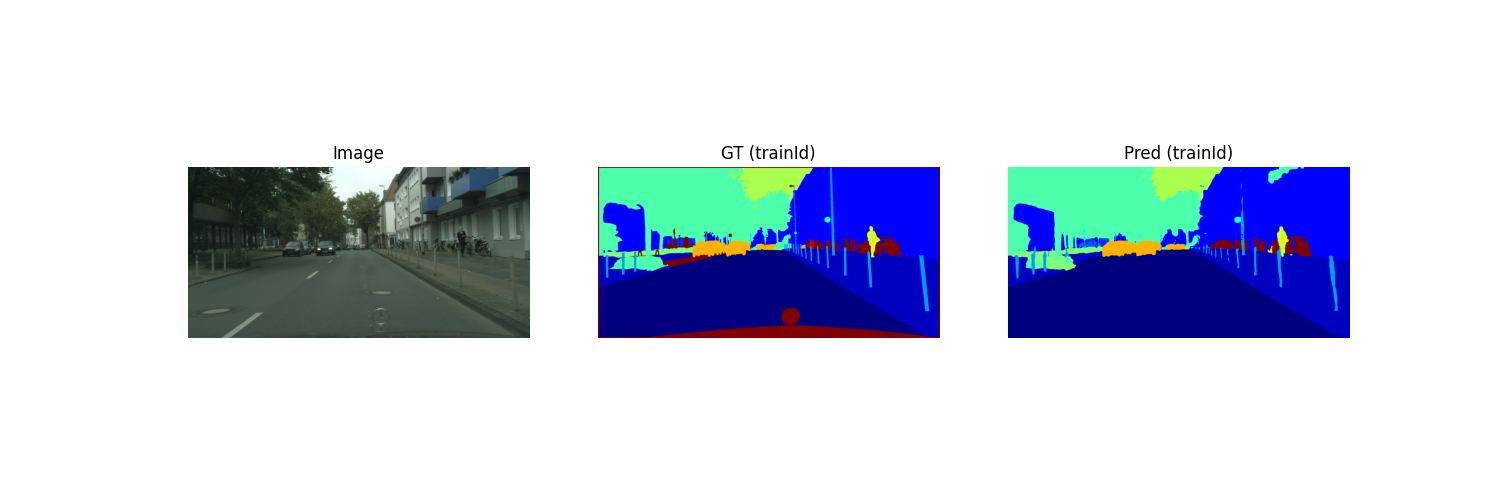
\includegraphics[width=0.9\linewidth]{../cała_praca/figures_auto/seg_0.png}
  \caption{Przykładowa segmentacja 1.}
\end{figure}

\begin{figure}[hbp]
  \centering
  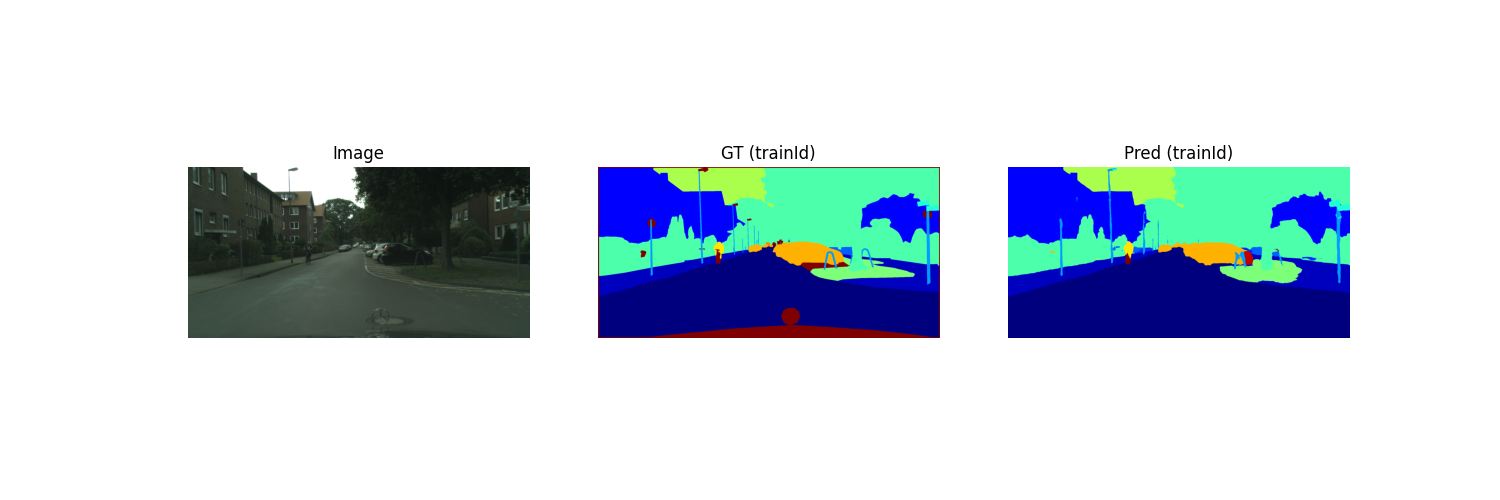
\includegraphics[width=0.9\linewidth]{../cała_praca/figures_auto/seg_1.png}
  \caption{Przykładowa segmentacja 2.}
\end{figure}

\begin{figure}[hbp]
  \centering
  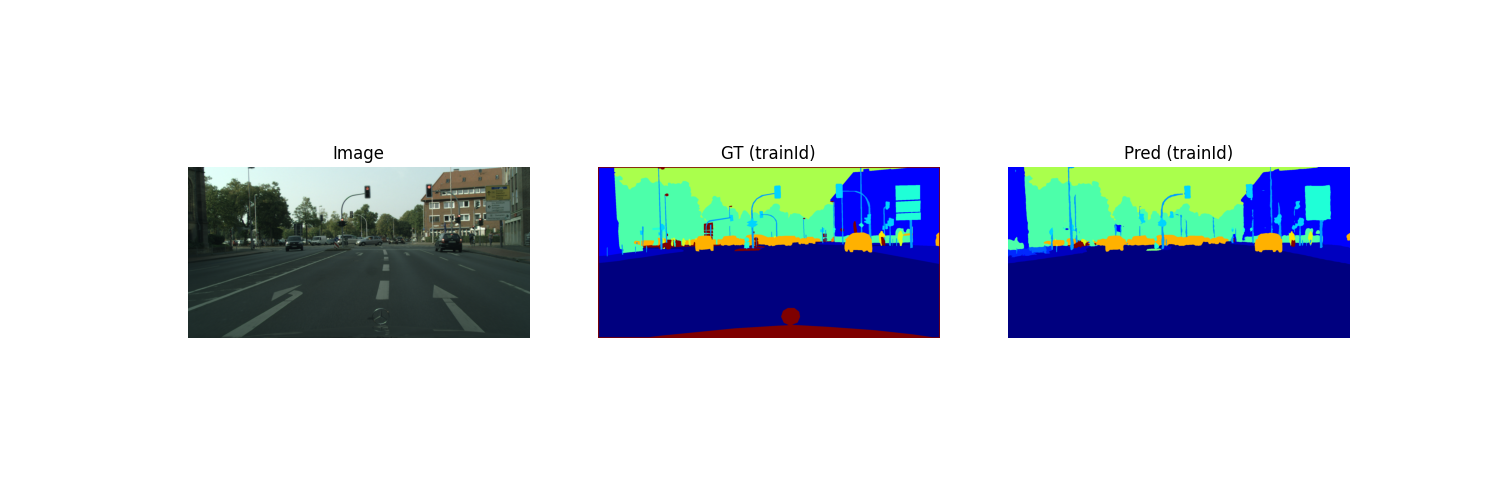
\includegraphics[width=0.9\linewidth]{../cała_praca/figures_auto/seg_2.png}
  \caption{Przykładowa segmentacja 3.}
\end{figure}

\begin{figure}[hbp]
  \centering
  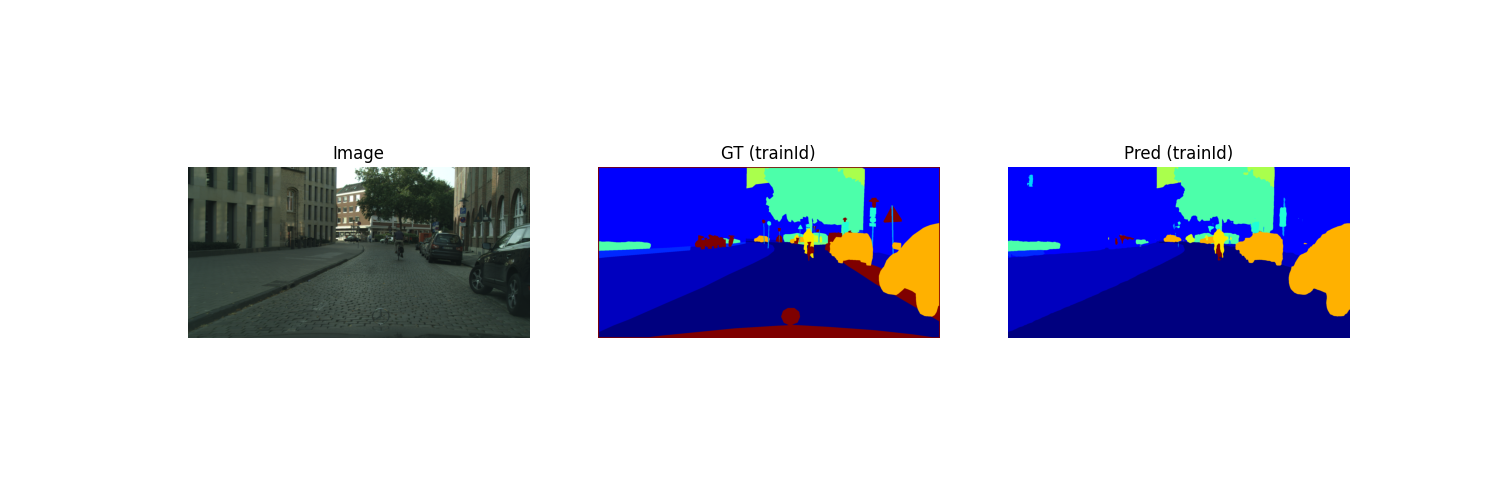
\includegraphics[width=0.9\linewidth]{../cała_praca/figures_auto/seg_3.png}
  \caption{Przykładowa segmentacja 4.}
\end{figure}

\end{document}
